\chapter{Approach and Implementation}
\label{ch:approach}

textwidth: \printinunitsof{in}\prntlen{\textwidth}

linewidth: \printinunitsof{in}\prntlen{\linewidth}

In this chapter the basic work flow is described in detail. The process is mainly drive by an exploratory approach, but follows primarily Farines and Whiteheads~\cite{farine2015constructing} primary steps and key considerations for social network analysis to non-human animal data. The adapted and resulting process is visualized in figure~\ref{fig:process}.

The dataset was first analysed regarding data quality and to form an understanding of the dataset and behaviour of bees in general. Those findings were used to define nodes and infer associations/edges to build the network, respectively derive parameters for the network-generating-pipeline. The static and temporal networks are analysed using network scienc tools and methods (e.g. XXX). For testing hypothesis the networks are combined with attributed data (positions and age information). Each step is explained within the following sections.

\begin{figure}[htb]
	\centering
	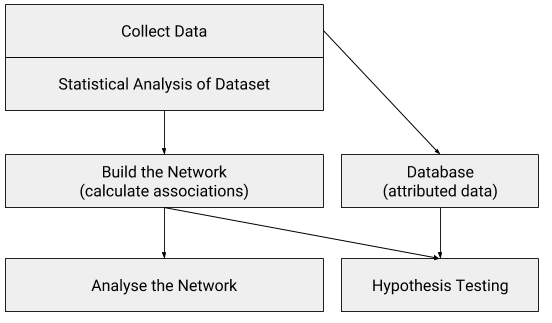
\includegraphics[width=1.0\textwidth]{Figures/WorkProcess}
	\caption{Steps of the Research Approach}
	\label{fig:process}
\end{figure}


\section{The Dataset}
\label{sec:dataset}
The basis of the dataset are video files, that capture tagged honey bees of one colony in a two sided observation hive.
Each individual of the colony, including about 3200 bees, were tagged with 12-bit markers. Four cameras were used to film the hive, the setup of the cameras is illustrated in figure~\ref{fig:cams} and an example of tagged bees is shown in figure~\ref{fig:markers}.

The recording season lastet nine weeks (63 days), around the clock, from 19.07.2016 until 19.09.2016, with some interruptions due to maintainance and technical failures, this is shown in figure~\ref{fig:period}.
The recording resolution of each camera is three frames per second, aiming for $1024$ frames (about $5.7$ minutes) for a video files.For each frame, bee detections were extracted by using an image analysis pipeline.

\begin{figure}[htb]
	\centering
	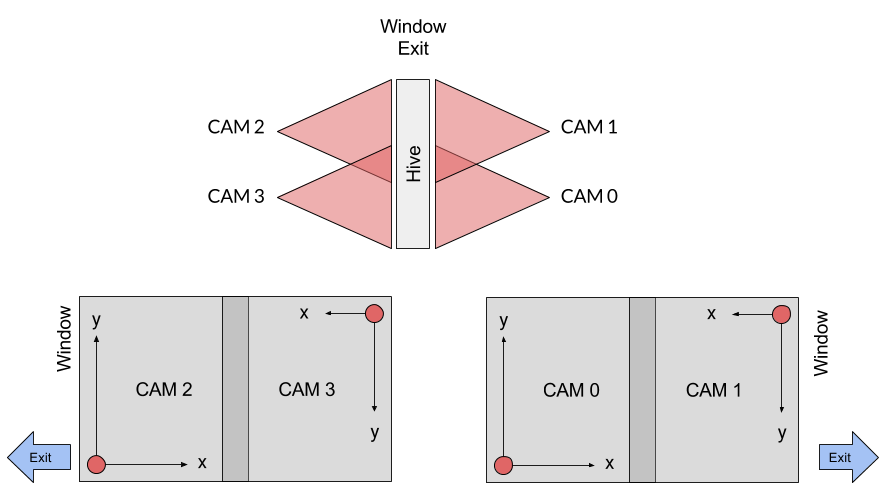
\includegraphics[width=1.0\textwidth]{Figures/setupCams}
	\caption{Camera Setup in 2016: (1) Top View:  vertical hive with two cameras for each side, overlapping in the middle. (2) Front View: left and right camera setup, the red dot indicated the origin $(0,0)$ of the camera.}
	\label{fig:cams}
\end{figure}

The resulting detection data is stored in a binary file format. A python library called \emph{bb-binary}\footnote{\url{https://github.com/BioroboticsLab/bb_binary}; Last accesed: 2106-02-16, 04:28PM} provides easy access to the binary files. Each file in bb\_binary file format corresponds to a video file of a single camera.
The size of the complete dataset for 2016 is $470$~GB, about $7.5$~GB of binary data per day.

In 2016 exactly $3.191$ bees were tagged. The tagging period is 67 days long. The tagging started on 2016-06-28 (22 days before the recording started) and lasted until 2016-09-02, so 17 days before the recording ended. The your bees were tagged and then added to the hive. The overall tagging frequency is shown in figure~\ref{fig:tagging}. The hatching day for each bee is known. On the day when the recording started about half of the tags were used up. 

\begin{figure}[htb]
	\centering
	
\includegraphics[width=0.5\textwidth]{Figures/foo}
	\caption{Recording Season with maintainance and failures}
	\label{fig:period}
\end{figure}

\begin{figure}[htb]
	\centering
	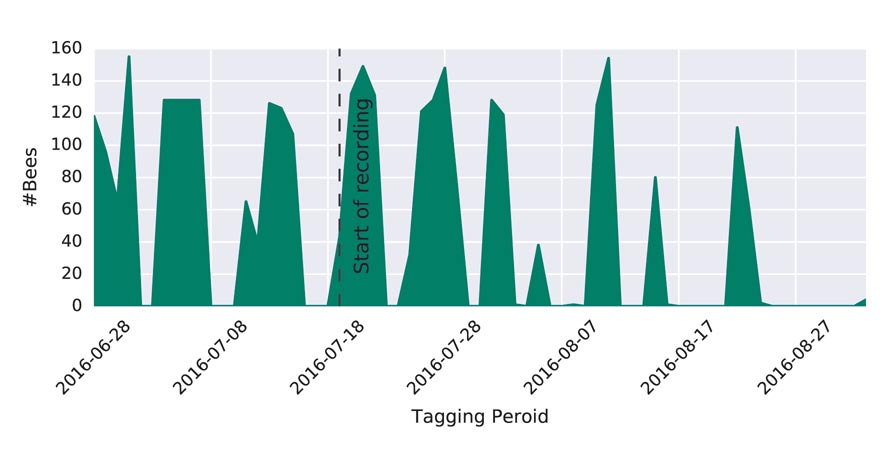
\includegraphics[width=1.0\textwidth]{Figures/tagging_period}
	\caption[Tagging Frequency]{Tagging frequency of bees: The bees were primarily tagged during the week. The weekend (sometimes also mondays or fridays) no bees were tagged. On average 48 bees were tagged each day, considering only tagging days, the average is about 91 ($\pm50$) bees (median 118, mode 128).}
	\label{fig:tagging}
\end{figure}

\subsection{Structure of the Dataset}
The data is organised in \emph{frame container}, wich corresponds to a video file of a single camera. A frame container holds all \emph{frames} for that specific video.
Each frame has a list of all bees detected by the image analysis pipeline.

A \emph{detection} has the following attributes, which are relevant to this project:

\begin{itemize}
\item \textbf{xpos}: $x$ coordinate of bee with respect to the image in pixel
\item \textbf{ypos}: $y$ coordinate of bee with respect to the image in pixel
\item \textbf{radius}: of the tag
\item \textbf{decodedId}: decoded 12-bit id, the bit probabilities are discretised to 0-255
\end{itemize}

Besides further information, the frame container specifies the camera and a frame is also attributed with a timestamp. The data can be accessed iterating on frame container (file) or on frame level, in both cases using timestamps for start and end. The data scheme is illustrated in figure~\ref{fig:scheme}.
The complete data scheme can be found on github\footnote{\url{https://github.com/BioroboticsLab/bb_binary/blob/master/bb_binary/bb_binary_schema.capnp}; Last accessed: 2106-02-16, 04:46PM}. 


\subsection{ID Confidence and Tracking Quality}
Each bit of the decoded 12-bit ID represents a probability between $0$ and $255$. That means when using a high ID confidence\footnote{The confidence of an ID is calculated as follows. TODO} results in less data, but with a higher accuracy, a low confidence on more data, but rather uncertain and errors. A good tradeoff between data quality and amount of data should be chosen. Figure~\ref{fig:tradeoff} shows the proportion of wrong detections depending on the confidence level for all four cameras. For a confidece level of $0.9$ wrong detection are about $4\%$, but the amount of data is still at $70\%$ (todo choose values according to figure).

\begin{figure}[htb]
	\centering
	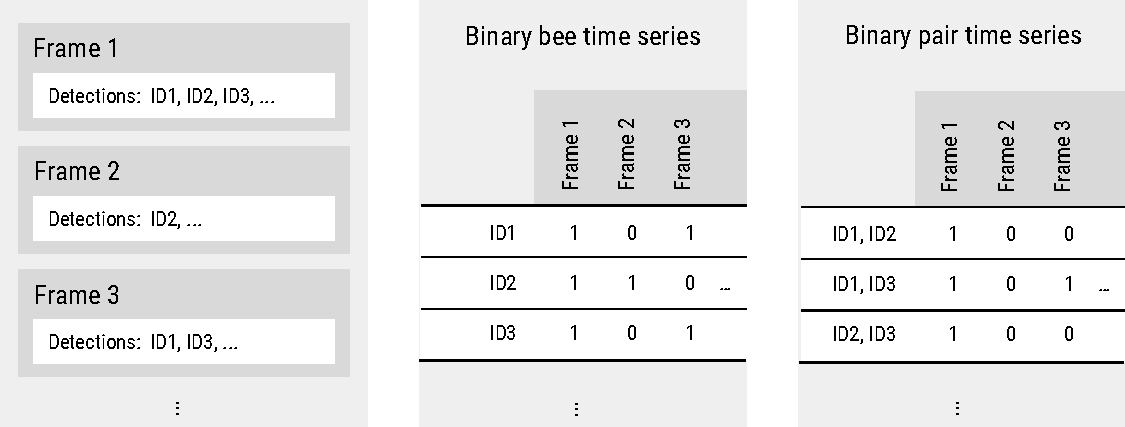
\includegraphics[width=1.0\textwidth]{Figures/structure}
	\caption{Structure of the data scheme}
	\label{fig:scheme}
\end{figure}

\begin{figure}[htb]
	\centering
	
\includegraphics[width=0.5\textwidth]{Figures/foo}
	\caption[Tradeoff: Confidence level, data quality and amount of data]{On 21.07.2016, about half of the bee tags were used up. This day was chosen to determine the effects of the ID confidence level on data quality and amount of remaining data. For each camera a ten minute test dataset was chosen (12:00-12:10) with a sample size of $10.000$. For each detected bee, the age was determined, negative ages were counted as wrong detection (dann mal zwei rechnen weil die falschen die rechts drin sind sieht man ja nicht, desswegen wurde die Haelfte gewaehlt.).}
	\label{fig:tradeoff}
\end{figure}

Some statistics about the tracking quality, gaps of size one, two, three and so on. This is relevant for later on. Damn!

\subsection{Some Statistics}
TODO
speed of bees\\
presence and absence of bees (counted and as duration)\\

\subsection{Implications}
TODO


\section{Inferring Networks}

\subsection{Network Pipeline}
\subsection{Thresholding Edges}
\subsection{Runtime and Complexity}

\section{Static and Temporal Analysis}	






